\documentclass[../../main/main.tex]{subfiles}
\graphicspath{{./figures/}}

\dominitoc
\faketableofcontents

\renewcommand{\mtcSfont}{\small\bfseries}
\renewcommand{\mtcSSfont}{\footnotesize}

\makeatletter
\renewcommand{\@chapapp}{Chimie -- chapitre}
\makeatother

% \toggletrue{student}
% \toggletrue{corrige}
% \renewcommand{\mycol}{black}
% \renewcommand{\mycol}{gray}

\hfuzz=5.002pt

\begin{document}
\setcounter{chapter}{5}

\settype{book}
\settype{prof}
\settype{stud}

\chapter{R\'eactions d'oxydo-r\'eduction}

\vspace*{\fill}

\begin{prgm}
	\small
	\begin{tcb}*(ror)"know"{Savoirs}
		\begin{itemize}
			\item Oxydants et réducteurs, réactions d'oxydoréduction, nombre
			      d'oxydation, dismutation et médiamutation.
			\item Exemples d'oxydants et de réducteurs minéraux usuels : nom, nature
			      et formule des ions thiosulfate, permanganate, hypochlorite, du
			      peroxyde d'hydrogène.
			\item Pile, tension à vide, potentiel d'électrode, formule de
			      \textsc{Nernst}, électrodes de référence.
			\item Diagrammes de prédominance ou d'existence.
			\item Aspect thermodynamique des réactions d'oxydo-réduction.
		\end{itemize}
	\end{tcb}
	\begin{tcb}*(ror)"how"{Savoir-faire}
		\begin{itemize}
			\item Relier la position d'un élément dans le tableau périodique et le
			      caractère oxydant ou réducteur du corps simple correspondant.

			\item Prévoir les nombres d'oxydation extrêmes d'un élément à partir de sa
			      position dans le tableau périodique.

			\item Identifier l'oxydant et le réducteur d'un couple.

			\item Décrire le fonctionnement d'une pile à partir d'une mesure de
			      tension à vide ou à partir des potentiels d'électrode.

			\item Utiliser les diagrammes de prédominance ou d'existence pour prévoir
			      les espèces incompatibles ou la nature des espèces majoritaires.

			\item Prévoir qualitativement ou quantitativement le caractère
			      thermodynamiquement favorisé ou défavorisé d'une réaction
			      d'oxydo-réduction à partir des potentiels standard des couples.
		\end{itemize}
	\end{tcb}
\end{prgm}

\vspace*{\fill}
\minitoc
\vspace*{\fill}

\newpage

\vspace*{\fill}
% {
\begin{boxes}
	\footnotesize
	\begin{tcb}(defi)<lftt>{Liste des définitions}
		\tcblistof[\paragraph*]{defi}{\hspace*{3pt}}
	\end{tcb}
	% \begin{tcb}(rapp)<lftt>{Liste des rappels}
	% 	\tcblistof[\paragraph*]{rapp}{\hspace*{3pt}}
	% \end{tcb}
	\begin{tcb}(prop)<lftt>{Liste des propriétés}
		\tcblistof[\paragraph*]{prop}{\hspace*{3pt}}
		% \tcblistof[\paragraph*]{loi}{\hspace*{3pt}}
		\tcblistof[\paragraph*]{theo}{\hspace*{3pt}}
	\end{tcb}
	% \begin{tcb}(coro)<lftt>{Liste des corollaires}
	% 	\tcblistof[\paragraph*]{coro}{\hspace*{3pt}}
	% \end{tcb}
	\begin{tcb}(demo)<lftt>{Liste des démonstrations}
		\tcblistof[\paragraph*]{demo}{\hspace*{3pt}}
		\tcblistof[\paragraph*]{prev}{\hspace*{3pt}}
	\end{tcb}
	% \begin{tcb}(inte)<lftt>{Liste des interprétations}
	% 	\tcblistof[\paragraph*]{inte}{\hspace*{3pt}}
	% \end{tcb}
	\begin{tcb}(tool)<lftt>{Liste des outils}
		\tcblistof[\paragraph*]{tool}{\hspace*{3pt}}
	\end{tcb}
	% \begin{tcb}(nota)<lftt>{Liste des notations}
	% 	\tcblistof[\paragraph*]{nota}{\hspace*{3pt}}
	% \end{tcb}
	\begin{tcb}(appl)<lftt>{Liste des applications}
		\tcblistof[\paragraph*]{appl}{\hspace*{3pt}}
	\end{tcb}
	% \begin{tcb}(rema)<lftt>{Liste des remarques}
	% 	\tcblistof[\paragraph*]{rema}{\hspace*{3pt}}
	% \end{tcb}
	% \begin{tcb}(exem)<lftt>{Liste des exemples}
	% 	\tcblistof[\paragraph*]{exem}{\hspace*{3pt}}
	% \end{tcb}
	\begin{tcb}(ror)<lftt>{Liste des points importants}
		\tcblistof[\paragraph*]{ror}{\hspace*{3pt}}
	\end{tcb}
	\begin{tcb}(impo)<lftt>{Liste des erreurs communes}
		\tcblistof[\paragraph*]{impo}{\hspace*{3pt}}
	\end{tcb}
\end{boxes}
% }
\vspace*{\fill}
\newpage

\section{Oxydants et réducteurs}

\subsection{Couples oxydo-réducteurs}
\begin{tcb*}(defi){Oxydant et réducteur}
	\begin{itemize}
		\bitem{Un oxydant} est une espèce chimique capable de \xul{\psw{capter}} un
		ou plusieurs électrons~;
		\bitem{Un réducteur} est une espèce chimique capable de \xul{\psw{céder}} un
		ou plusieurs électrons~;
		\bitem{Un couple} oxydant-réducteur, noté Ox/Red\ftn{On fera donc
			particulièrement au sens qui n'est pas «~rédox~»~!}, est associé
		\textit{via} la \textbf{demi-équation} électronique~:
		\psw{
			\[
				\ce{Red} \ce{=} \ce{Ox} + ne^-
			\]
		}
		\vspace{-15pt}
	\end{itemize}
\end{tcb*}
\begin{tcb*}(exem)<lftt>{Couples simples}
	\begin{itemize}
		\item
		      \leftcentersright{%
		      Le cuivre~:
		      }{%
		      \psw{$\ce{Cu_{\rm(s)} = Cu^2+_{\rm(aq)} + 2e^-}$}
		      }{%
		      % \ce{Cu^2+} est un \xul{\psw{oxydant}}, \ce{Cu} est un \xul{\psw{réducteur}}
		      \ce{Cu^2+} \xul{\psw{oxydant}}, \ce{Cu} \xul{\psw{réducteur}}
		      }%
		      \vspace{-12pt}
		\item
		      \leftcentersright{%
		      Le zinc~:
		      }{%
		      \psw{$\ce{Zn_{\rm(s)} = Zn^2+_{\rm(aq)} + 2e^-} $}
		      }{%
		      De même
		      }%
		      \vspace{-12pt}
		\item
		      \leftcentersright{%
		      Le dichlore~:
		      }{%
		      \psw{$\ce{2Cl^-_{\rm(aq)} = Cl_2_{\rm(g)} + 2e^-} $}
		      }{%
		      \ce{Cl2} \xul{\psw{oxydant}}, \ce{Cl^-} \xul{\psw{réducteur}}
		      }
	\end{itemize}
\end{tcb*}

\begin{tcb*}(tool){Équilibrer une demi-réaction}
	Pour équilibrer une demi-équation en \textbf{milieu acide}~:
	\begin{enumerate}[label=\sqenumi]
		\item Équilibrer les éléments \textbf{autres que \ce{O} ou \ce{H}}~;
		\item Équilibrer \textbf{l'oxygène avec $\ce{H2O}_{\rm(l)}$}~;
		\item Équilibrer \textbf{les hydrogènes avec $\ce{H+_{\rm(aq)}}$}~;
		\item Équilibrer \textbf{les charges avec $e^-$}
	\end{enumerate}
	Si le \textbf{milieu est basique}, écrire une équation avec des
	$\ce{{H}^+_{\rm(aq)}}$ n'est pas représentatif de la réalité~:
	\begin{enumerate}[label=\sqenumi, resume]
		\item On \textbf{remplace \ce{H+} par \ce{HO-}} grâce à l'autoprotolyse de
		      l'eau~:
		      \[
			      \ce{H_2O_{\rm(s)} = H^+_{\rm(aq)} + HO^-_{\rm(aq)}}
		      \]
	\end{enumerate}
\end{tcb*}

\begin{tcb*}[breakable](appl)<lftt>{Équilibrage d'une équation rédox}
	\begin{enumerate}
		\item   Équilibrer la demi-équation du couple
		      $\ce{{MnO_4}^-_{\rm(aq)}}/\ce{MnO_2_{\rm(s)}}$ en milieu basique.
		\item Équilibrer la demi-équation du couple
		      $\ce{{Cr_2O_7}^2-_{\rm(aq)}}/\ce{{Cr}^3+_{\rm(aq)}}$
	\end{enumerate}
	\tcblower
	\begin{enumerate}
		\item
		      \leavevmode\vspace*{-25pt}\relax
		      \begin{align*}
			      \beforetext{\fbox{1}}
			      \psw{\ce{MnO_2_{\rm(s)}}}
			       & =
			      \psw{\ce{{MnO_4}^-_{\rm(aq)}}}
			      \tag*{}
			      \\\beforetext{\fbox{2}}
			      \psw{\ce{MnO_2_{\rm(s)} + 2H_2O_{\rm(l)}}}
			       & =
			      \psw{\ce{{MnO_4}^-_{\rm(aq)}}}
			      \\\beforetext{\fbox{3}}
			      \psw{\ce{MnO_2_{\rm(s)} + 2H_2O_{\rm(l)}}}
			       & =
			      \psw{\ce{{MnO_4}^-_{\rm(aq)} + 4 {H}^+_{\rm(aq)}}}
			      \\\beforetext{\fbox{4}}
			      \psw{\ce{MnO_2_{\rm(s)} + 2H_2O_{\rm(l)}}}
			       & =
			      \psw{\ce{{MnO_4}^-_{\rm(aq)} + 4 {H}^+_{\rm(aq)} + 3e^-}}
			      \tag*{\llap{milieu acide}}
			      \\\beforetext{\fbox{5}}
			      \psw{\ce{MnO_2_{\rm(s)} + 4HO^-_{\rm(aq)}}}
			       & =
			      \psw{\ce{{MnO_4}^-_{\rm(aq)} + 2H_2O_{\rm(l)} + 3e^-}}
			      \tag*{\llap{milieu basique}}
		      \end{align*}
		      \newpage
		\item
		      \leavevmode\vspace*{-25pt}\relax
		      \begin{align*}
			      \beforetext{\fbox{1}}
			      \psw{\ce{2 {Cr}^3+_{\rm(aq)}}}
			       & =
			      \psw{\ce{{Cr_2O_7}^2-_{\rm(aq)}}}
			      \tag*{}
			      \\\beforetext{\fbox{2}}
			      \psw{\ce{2 {Cr}^3+_{\rm(aq)} + 7 {H_2O}_{\rm(l)}}}
			       & =
			      \psw{\ce{{Cr_2O_7}^2-_{\rm(aq)}}}
			      \\\beforetext{\fbox{3}}
			      \psw{\ce{2 {Cr}^3+_{\rm(aq)} + 7 {H_2O}_{\rm(l)}}}
			       & =
			      \psw{\ce{{Cr_2O_7}^2-_{\rm(aq)} + 14 {H}^+_{\rm(aq)}}}
			      \\\beforetext{\fbox{4}}
			      \psw{\ce{2 {Cr}^3+_{\rm(aq)} + 7 {H_2O}_{\rm(l)}}}
			       & =
			      \psw{\ce{{Cr_2O_7}^2-_{\rm(aq)} + 14 {H}^+_{\rm(aq)} + 6e^-}}
			      \tag*{\llap{milieu acide}}
			      \\\beforetext{\fbox{5}}
			      \psw{\ce{2 {Cr}^3+_{\rm(aq)} + 14 {HO}^-_{\rm(aq)}}}
			       & =
			      \psw{\ce{{Cr_2O_7}^2-_{\rm(aq)} + 7 {H_2O}_{\rm(l)} + 6e^-}}
			      \tag*{\llap{milieu basique}}
		      \end{align*}
	\end{enumerate}
\end{tcb*}

\begin{tcb*}*[sidebyside](exem)<lftt>"ror"{Couples à connaître}
	\small
	\begin{itemize}
		\item Ions tétrathionate/ion thiosulfate
		      \psw{
		      \[
			      \ce{{2S_2O_3}^2-_{\rm(aq)} = {S_4O_6}^2-_{\rm(aq)} + 2e^-}
		      \]
		      }
		      \vspace{-20pt}
		\item Ion permanganate/ion manganèse \myRoman{2}
		      \psw{
		      \[
			      \ce{
			      {Mn}^2+_{\rm(aq)} + 4H_2O_{\rm(l)}
				      =
				      {MnO_4}^-_{\rm(aq)} + 8H^+_{\rm(aq)} + 5e^-
			      }
		      \]
		      }
		      \vspace{-20pt}
		\item Ion hypochlorite/ion chlorure
		      \psw{
		      \[
			      \ce{
			      {Cl}^-_{\rm(aq)} + {H_2O}_{\rm(l)}
				      =
				      {ClO}^-_{\rm(aq)} + 2 {H}^+_{\rm(aq)} +2e^-
			      }
		      \]
		      }
		      \vspace{-20pt}
		\item Ion dichromate/ion chrome \myRoman{3}
		      \psw{
		      \[
			      \ce{
			      2 {Cr}^3+_{\rm(aq)} + 7H_2O_{\rm(l)}
				      =
				      {Cr_2O_7}^2-_{\rm(aq)} + {14H}^+_{\rm(aq)} + 6e^-
			      }
		      \]
		      }
	\end{itemize}
	\vspace{-30pt}
	\tcblower
	\small
	\begin{itemize}
		\item Peroxyde d'hydrogène\ftn{Aussi appelée «~eau oxygénée~»}/eau
		      \psw{
		      \[
			      \ce{
			      2 {H_2O}_{\rm(l)}
				      =
				      {H_2O_2}_{\rm(aq)} + 2 {H}^+_{\rm(aq)} + 2e^-
			      }
		      \]
		      }
		      \vspace{-20pt}
		\item dioxygène/eau
		      \psw{
		      \[
			      \ce{
			      2 {H_2O}_{\rm(l)}
				      =
				      {O_2}_{\rm(g)} + 4 {H}^+_{\rm(aq)} +4 e^-
			      }
		      \]
		      }
		      \vspace{-20pt}
		\item dioxygène/peroxyde d'hydrogène
		      \psw{
		      \[
			      \ce{
			      {H_2O_2}_{\rm(aq)}
				      =
				      {O_2}_{\rm(g)} + 2 {H}^+_{\rm(aq)} +2 e^-
			      }
		      \]
		      }
		      \vspace{-20pt}
		\item Eau/dihydrogène
		      \psw{
		      \[
			      \ce{
			      {H_2}_{\rm(g)}
			      =
			      2 {H}^+_{\rm(aq)} + 2e^-
			      }
		      \]
		      }
	\end{itemize}
	\vspace{-30pt}
\end{tcb*}

\begin{tcb*}(rema)<lftt>{Autour des demi-équations}
	\begin{itemize}
		\item Ces demi-équation ne représentent pas de réelles transformations
		      chimiques, on ne peut faire intervenir explicitement des électrons
		      libres~: ce sont des outils.
		\item Comme pour les réactions acide-base, certaines espèces sont à la fois
		      oxydante et réductrice.
		      % \item Il est parfois évident de déterminer l'oxydant d'un couple par
		      %       l'écriture de la demi-équation de, mais parfois non. On va développer
		      %       un critère qui s'applique de manière plus générale.
	\end{itemize}
\end{tcb*}

\subsection{Nombre d'oxydation}

\begin{tcb*}(defi){Nombre d'oxydation}
	Le \textbf{nombre d'oxydation}\ftn{Aussi \textbf{degré d'oxydation}} d'un
	\textbf{atome dans une molécule} est le nombre de charges élémentaires $e$
	qu'il porterait si on venait à répartir les électrons des liaisons aux
	\textbf{plus électronégatifs}. Il s'écrit en \xul{chiffres romains}.
\end{tcb*}

\begin{tcb*}[sidebyside, sidebyside align=top](exem)<lftt>
		{Illustrations simples du nombre d'oxydation}
	\begin{itemize}
		\bitem{Oxygène dans dioxygène}~:
		\begin{center}
			\sswitch{
				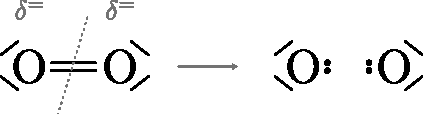
\includegraphics[width=0.7\linewidth, draft=true]{no_O-O2.pdf}
			}{
				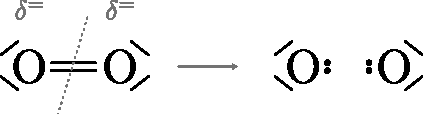
\includegraphics[width=0.7\linewidth]{no_O-O2.pdf}
			}
		\end{center}
		\psw{
			Après répartition fictive des électrons, chaque oxygène est neutre~: $\no{O}
				= 0$
		}
	\end{itemize}
	\vspace{-30pt}
	\tcblower
	\begin{itemize}
		\bitem{Oxygène et hydrogène dans l'eau}~:
		\begin{center}
			\sswitch{
				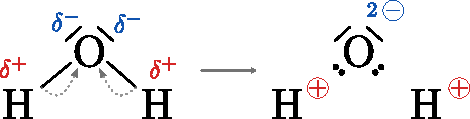
\includegraphics[width=0.7\linewidth, draft=true]{no_O-H2O.pdf}
			}{
				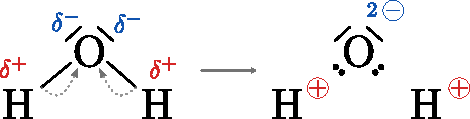
\includegraphics[width=0.7\linewidth]{no_O-H2O.pdf}
			}
		\end{center}
		\psw{
			Après la répartition fictive des électrons,
			% $q_{\ce{O}} = -2e$ et $q_{\ce{H}} = +e$
			$\no{O} = -\myRoman{2} \qqet \no{H} = +\myRoman{1}$
		}
	\end{itemize}
	\vspace{-30pt}
\end{tcb*}

\begin{tcb*}(prop){Nombre d'oxydation}
	\begin{itemize}
		\item Le nombre d'oxydation d'un élément est lié à \textbf{sa structure
			      électronique}~: dans un édifice chaque élément cherche à se
		      rapprocher de la structure des gaz nobles en remplissant ou vidant
		      sa couche de valence, et son nombre d'oxydation est donc
		      \textbf{borné}.
		\item Lors d'une \textbf{oxydation}, \textbf{\no $\nearrow$}~; lors d'une
		      \xul{réduction}, \xul{\no $\searrow$}.
	\end{itemize}
\end{tcb*}

\begin{tcb*}[sidebyside, righthand ratio=.45](exem)<lftt>{Nombre d'oxydation et structure électronique}
	\begin{itemize}
		\bitem{Oxygène}~: \psw{$\chi_{\ce{O}} \nearrow \quad \Ra \quad$ souvent
			chargé $-2e$}
		\bitem{Alcalins}~: \psw{facilement +\myRoman{1}}
		\bitem{Alcalinos-terreux}~: \psw{facilement +\myRoman{2}}
		\bitem{Halogènes}~: \psw{facilement -\myRoman{1}}
		\bitem{Gaz nobles}~: \psw{pas d'oxydation ou de réduction}
	\end{itemize}
	\tcblower
	\begin{center}
		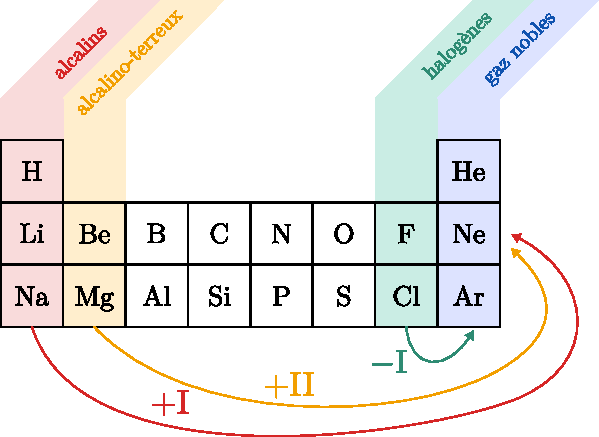
\includegraphics[width=\linewidth]{no_tab.pdf}
	\end{center}
\end{tcb*}

\begin{tcb*}(ror){Règles de calcul nombre d'oxydation}
	\begin{enumerate}
		\item Le \no d'un élément seul est égal à sa charge~;
		\item La somme des \no des élements d'une molécule est égale à la charge
		      de la molécule~;
		      % \item Les éléments d'ions et de molécules homonucléaires ont le même nombre
		      %   d'oxydation de l'élément (???)
		\item En général, dans les molécules et ions complexes, $\no{H} =
			      +\myRoman{1}$~;
		\item En général, dans les molécules et ions complexes, $\no{O} =
			      -\myRoman{2}$ (sauf si cela met en défaut les règles précédentes).
	\end{enumerate}
\end{tcb*}

\begin{tcb*}[sidebyside, lefthand ratio=.26](appl)<lftt>{Calculs de nombres d'oxydation}
	\small
	\begin{itemize}
		\item \ce{Cu}~: \psw{$\no{Cu} = 0$}
		\item \ce{Cu^2+}~: \psw{$\no{Cu} = +\myRoman{2}$}
		\item \ce{Fe^3+}~: \psw{$\no{Fe} = +\myRoman{3}$}
	\end{itemize}
	\tcblower
	\small
	\begin{itemize}
		\item \ce{H2O2}~: \psw{$\no{H} = +\myRoman{1} \Ra 2 \cdot 1 + 2 \cdot
				      \no{O} = 0 \Lra \no{O} = - \myRoman{1}$}
		\item \ce{IO3^-}~: \psw{$\no{O} = -\myRoman{2} \Ra \no{I}+3 \cdot (-2) =
				      -1 \Lra \no{I} = +\myRoman{5}$}
		\item \ce{S2O3^2-}~: \psw{$\no{O} = -\myRoman{2} \Ra 2 \cdot \no{S}+ 3
				      \cdot (-2) = -2 \Ra \no{S} = +\myRoman{2}$}
	\end{itemize}
\end{tcb*}

\begin{tcb}*(expe)<itc>"trans"{Transition}
	Ainsi, l'équilibre entre les espèces d'un couple repose sur la capacité du
	milieu à recevoir ou perdre des électrons~: les couples oxydant-réducteur ont
	donc des caractéristiques électriques.
\end{tcb}

\section{Distribution des espèces d'un couple}
\subsection{Potentiel d'un couple}

\begin{tcb*}[breakable](prop){Formule de \textsc{Nernst}}
	Pour une demi-équation d'oxydoréduction
	\psw{
	\[
		\ce{\alpha Red + \beta H_2O_{\rm(l)} = \gamma Ox + \delta {H}^+_{\rm(aq)} +}
		ne^-
	\]
	}
	le potentiel électrique d'une solution à l'équilibre est donné par la formule
	de \textsc{Nernst}~:
	\psw{
		\[
			E(\ce{Ox}/\ce{Red}) = E^\circ(\ce{Ox}/\ce{Red}) +
			\frac{RT}{n\Fc} \ln
			\frac{a_{\ce{Ox}}^{\gamma}[\ce{H+}]^{\delta}}
			{a_{\ce{Red}}^{\alpha}{c^\circ}^{\delta}}
		\]
	}
	\vspace{-20pt}
	\begin{itemize}
		\item $E$ est le potentiel, et s'exprime en \xul{\psw{volts}}~;
		\item $E^\circ$ est le potentiel standard du couple à la température $T$~;
		\item $n$ le nombre d'électrons échangés (variation du degré d'oxydation)~;
		\item $R$ la constante des gaz parfaits en \xul{\psw{\si{J.K^{-1}.mol^{-1}}}}~;
		\item $T$ la température en \xul{\psw{kelvins}}~;
		\item $\Fc$ la constante de \textsc{Faraday}, représentant la charge
		      électrique d'une mole de protons~:
		      \psw{
			      \[
				      \Fc = e \Nc_A = \SI{96485}{C.mol^{-1}}
				      \quad \Ra \quad
				      \boxed{\frac{RT}{\Fc}\ln 10 \approx \SI{0.059}{V}}
			      \]
		      }
		      \vspace{-30pt}
	\end{itemize}
	D'où la forme commune~:
	\psw{
		\[
			\boxed{
				E(\ce{Ox}/\ce{Red}) = E^\circ(\ce{Ox}/\ce{Red}) +
				\frac{\num{0.06}}{n} \log
				\frac{a_{\ce{Ox}}^{\gamma}[\ce{H+}]^{\delta}}
				{a_{\ce{Red}}^{\alpha}{c^\circ}^{\delta}}
			}
		\]
	}
	\vspace{-15pt}
\end{tcb*}

\begin{tcb*}(rema)<lftt>{Autour de la formule de \textsc{Nernst}}
	\begin{itemize}
		\item Faites attention au passage du logarithme en base $e$ ($\ln$) au
		      logarithme décimal~:
		      \[
			      \log x = \frac{\ln x}{\ln 10}
		      \]
		\item Le potentiel seul n'a pas de sens de manière absolue~: il est défini
		      à une constante près. Il faut donc choisir une référence arbitraire afin
		      de fixer toutes les valeurs. On choisit pour cela le premier couple de
		      l'eau
		      \[
			      E^\circ(\ce{{H}^+_{\rm(aq)}}/\ce{{H_2}_{\rm(g)}}) = \SI{0}{V}
		      \]
	\end{itemize}
\end{tcb*}

\begin{tcb*}[breakable](appl)<lftt>{Calcul de potentiels}
	Donner les potentiels des couples suivants~:
	\begin{itemize}
		\item
		      \leftcenters{%
		      $\ce{{Fe}^2+_{\rm(aq)}}/\ce{Fe_{\rm(s)}}$~:
		      }{%
		      \psw{$\ce{Fe_{\rm(s)} = {Fe}^2+_{\rm(aq)} + 2e^-}$}
		      }
		      \vspace{-15pt}
		      \psw{
			      \[
				      E = E^\circ \left( \ce{Fe^2+}/\ce{Fe} \right) +
				      \frac{\num{0.06}}{2} \log \frac{[\ce{Fe^2+}]}{c^\circ}
			      \]
		      }
		      \vspace{-15pt}
		\item
		      \leftcenters{%
		      $\ce{{Fe}^3+_{\rm(aq)}}/\ce{{Fe}^2+_{\rm(aq)}}$~:
		      }{%
		      \psw{$\ce{{Fe}^2+_{\rm(aq)} = {Fe}^3+_{\rm(aq)} + e^-}$}
		      }
		      \vspace{-15pt}
		      \psw{
			      \[
				      E = E^\circ \left( \ce{Fe^3+}/\ce{Fe^2+} \right) +
				      \num{0.06} \log (\frac{[\ce{Fe^3+}]}{[\ce{Fe^2+}]})
			      \]
		      }
		      \vspace{-15pt}
		\item
		      \leftcenters{%
		      $\ce{{MnO_4}^-_{\rm(aq)}/\ce{{Mn}^2+_{\rm(aq)}}}$~:
		      }{%
		      \psw{
		      $\ce{
			      {Mn}^2+_{\rm(aq)} + 4 H_2O_{\rm(l)}
				      =
				      {MnO_4}^-_{\rm(aq)} + 8 {H}^+_{\rm(aq)} + 5e^-
			      }$
		      }
		      }
		      \vspace{-15pt}
		      \psw{
			      \[
				      E = E^\circ \left( \ce{{MnO_4}^-/\ce{{Mn}^2+}} \right) +
				      \frac{\num{0.06}}{5} \log ( \frac{[\ce{MnO_4^-}][\ce{H+}]^8}{[\ce{Mn^2+}]})
			      \]
		      }
		      \vspace{-15pt}
		\item
		      \leftcenters{%
		      $\ce{{H}^+_{\rm(s)}/\ce{H_2_{\rm(g)}}}$~:
		      }{%
		      \psw{$\ce{H_2_{\rm(g)} = 2 {H}^+_{\rm(aq)} + 2e^-}$}
		      }
		      \vspace{-15pt}
		      \psw{
			      \[
				      E = E^\circ \left( \ce{H+}/\ce{H_2} \right) +
				      \frac{\num{0.06}}{2} \log ( \frac{[H^+]^2p^\circ}{p_{\ce{H_2}}})
			      \]
		      }
		      \vspace{-15pt}
	\end{itemize}
\end{tcb*}

\subsection{Diagramme de prédominance}
\begin{tcb*}(ror){Diagramme de prédominance}
	\vspace{-10pt}
	\begin{gather*}
		\beforetext{Pour}
		\psw{
			\ce{\alpha Red = \gamma Ox} + n\ce{e^-}
		}
		\qqMath{on a}
		\psw{
			E = E^\circ(\ce{Ox}/\ce{Red}) + \frac{\num{0.06}}{n} \log
			(\frac{a_{\ce{Ox}}^{\gamma}}{a_{\ce{Red}}^{\alpha}})
		}
	\end{gather*}
	On utilisera alors une \textbf{convention de tracé} donnant la valeur de
	$\DS (a_{\ce{Ox}}^{\gamma})/(a_{\ce{Red}}^{\alpha})$ à la limite pour
	trouver $E\ind{lim}$, afin de tracer le diagramme de prédominance~:
	\vspace{-15pt}
	\begin{center}
		\sswitch{
			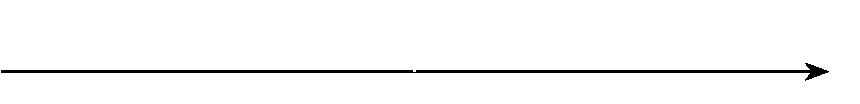
\includegraphics[width=\linewidth]{predom_plain}
		}{
			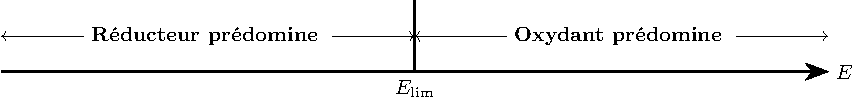
\includegraphics[width=\linewidth]{predom}
		}
		\vspace{-15pt}
		\captionof{figure}{Diagramme de prédominance générique}
	\end{center}
	% \begin{itemize}
	% 	\item à haut potentiel, \xul{\psw{l'oxydant}} domine~;
	% 	\item à bas potentiel, \xul{\psw{le réducteur}} domine.
	% \end{itemize}
\end{tcb*}
\begin{tcb*}(impo){Utilisation des diagrammes rédox}
	Ce raisonnement n'est valable \textbf{que pour un couple simple}, sans autres
	espèces dans la demi-réaction. À partir du moment où les protons \ce{H^+}
	interviennent, les diagrammes seront à 2 dimensions~: ce sont les
	\textbf{diagrammes potentiel-pH} (cf.\ chapitre suivant).
\end{tcb*}

\begin{tcb*}[breakable, sidebyside, righthand ratio=.25](defi){Force des oxydants et des réducteurs}
	Comme dans le cas des couples acide-base, on peut parler de la force d'un
	oxydant ou d'un réducteur selon la valeur du potentiel standard~:
	\begin{center}
		\begin{tabular}{ccc}
			\toprule
			$E^\circ$ & \textbf{Oxydant} & \textbf{Réducteur}
			\\
			Élevé     & \psw{fort}       & \psw{faible}
			\\
			Bas       & \psw{faible}     & \psw{fort}
			\\
			\bottomrule
		\end{tabular}
	\end{center}
	\tcblower
	\begin{center}
		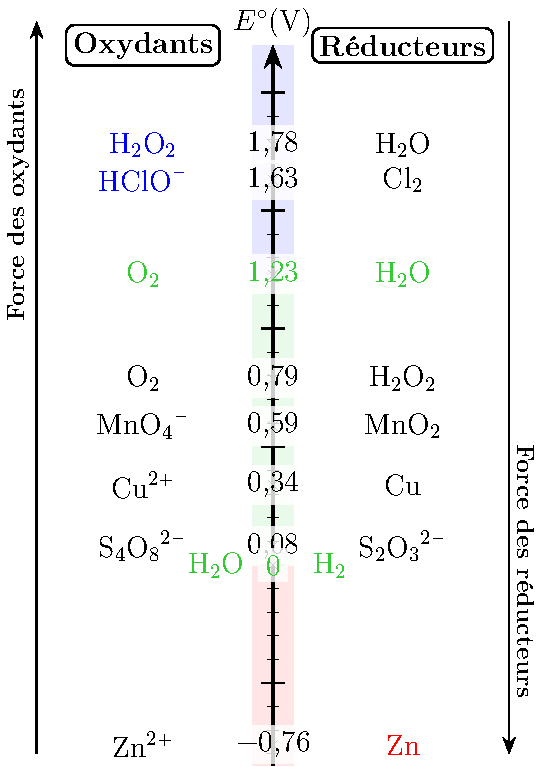
\includegraphics[width=\linewidth]{estand_scale}
		\captionsetup{justification=centering}
		\captionof{figure}{\\Échelle des $E^\circ$}
	\end{center}
\end{tcb*}

\section{Réactions entre couples}
\subsection{Réactions d'oxydoréduction}
\begin{tcb*}[breakable](defi){Réaction d'oxydoréduction}
	Une réaction d'oxydoréduction est une réaction de \textbf{transfert
		d'électrons} entre deux espèces~:
	\psw{
		\[
			\ce{Ox_1 + Red_2 = Red_1 + Ox_2}
		\]
	}
	\vspace{-25pt}
	\begin{itemize}
		\item L'oxydant \xul{\psw{capte}} un (des) électrons, il subit une
		      \xul{\psw{réduction}} et son \no \xul{\psw{diminue}}~;
		\item Le réducteur \xul{\psw{cède}} un (des) électrons, il subit une
		      \xul{\psw{oxydation}} et son \no \xul{\psw{augmente}}.
	\end{itemize}
\end{tcb*}

\begin{tcb*}(impo){Réactions d'oxydoréduction}
	\begin{itemize}
		\item Il n'y a jamais d'électrons dans la réaction bilan~;
		\item La somme des \no est conservée pendant une réaction rédox.
	\end{itemize}
\end{tcb*}

\begin{tcb*}(exem)<lftt>{Équilibrage d'équations rédox}
	\begin{enumerate}
		\item Écrire et équilibrer la réaction entre $\ce{{Fe}^3+_{\rm(aq)}}$ et
		      $\ce{Cu_{\rm(s)}}$. Les couples mis en jeu sont
		      $\ce{{Cu}^2+_{\rm(aq)}}/\ce{Cu_{\rm(s)}}$ et
		      $\ce{{Fe}^3+_{\rm(aq)}}/\ce{{Fe}^2+_{\rm(aq)}}$.
		\item Écrire et équilibrer la réaction entre $\ce{{Fe}^2+_{\rm(aq)}}$ et
		      $\ce{{MnO_4}^-_{\rm(aq)}}$. Les couples mis en jeu sont
		      $\ce{{MnO_4}^-_{\rm(aq)}}/\ce{{Mn}^2+_{\rm(aq)}}$ et
		      $\ce{{Fe}^3+_{\rm(aq)}}/\ce{{Fe}^2+_{\rm(aq)}}$
	\end{enumerate}
	\tcblower
	\begin{enumerate}
		\item \psw{
			      On écrit les deux demi-équations~:
			      \begin{align*}
				      \ce{Cu_{\rm(s)}}
				       & =
				      \ce{{Cu}^2+_{\rm(aq)} + 2e^-}
				      \tag{1}
				      \\
				      \ce{{Fe}^2+_{\rm(aq)}}
				       & =
				      \ce{{Fe}^3+_{\rm(aq)} + e^-}
				      \tag{2}
				      \\\beforetext{$(1) - 2 \cdot (2) \Ra$}
				      \Aboxed{
				      \ce{2 {Fe}^3+_{\rm(aq)} + Cu_{\rm(s)}}
				       & =
				      \ce{{Cu}^2+_{\rm(aq)} + 2 {Fe}^2+_{\rm(aq)}}
				      }
			      \end{align*}
		      }
		      \vspace{-15pt}
		\item \psw{
			      On écrit les deux demi-équations~:
			      \begin{align*}
				      \ce{{Mn}^2+_{\rm(aq)} + 4 H_2O_{\rm(l)}}
				       & =
				      \ce{{MnO_4}^-_{\rm(aq)} + 8 {H}^+_{\rm(aq)} + 5e^-}
				      \tag{1}
				      \\
				      \ce{{Fe}^2+_{\rm(aq)}}
				       & =
				      \ce{{Fe}^3+_{\rm(aq)} + e^-}
				      \tag{2}
				      \\\beforetext{$5 \cdot (2) - (1) \Ra$}
				      \Aboxed{
				      \ce{5{Fe}^2+_{\rm(aq)} + {MnO_4}^-_{\rm(aq)} + 8{H}^+_{\rm(aq)}}
				       & =
				      \ce{5 {Fe}^3+_{\rm(aq)} + {Mn}^2+_{\rm(aq)} + 4 H_2O_{\rm(l)}}
				      }
			      \end{align*}
		      }
		      \vspace{-15pt}
	\end{enumerate}
\end{tcb*}

\subsection{Sens de réaction}
Ainsi, comme pour les réactions acide-base, on peut déterminer la stabilité de
certains ions en solution, que ce soit par la superposition des diagrammes de
prédominance ou par la règle du gamma sur une échelle en $E^\circ$~:

\begin{tcb*}[sidebyside, righthand ratio=.25](ror){Sens spontané de réaction}
	Au cours d'une réaction d'oxydoréduction, l'\textbf{oxydant le plus fort} (de
	$E^\circ$ le plus élevé) réagit avec le \textbf{réducteur le plus fort} (de
	$E^\circ$ le plus faible). Cette règle schématise avec la \textbf{règle du
		gamma}, voir Figure~\ref{fig:gamma}.
	\smallbreak
	Cela se détermine aussi avec un diagramme de
	prédominance. En effet, deux espèces de \textbf{domaines disjoints} vont
	réagir ensemble pour donner les espèces qui peuvent exister ensemble au même
	potentiel, voir Figure~\ref{fig:disjoint}.
	\begin{center}
		\sswitch{
			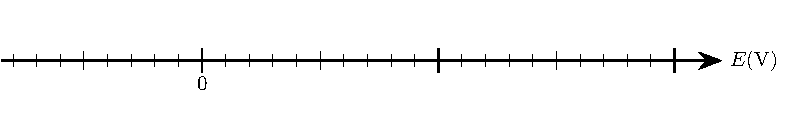
\includegraphics[width=\linewidth]{predom_2-plain}
		}{
			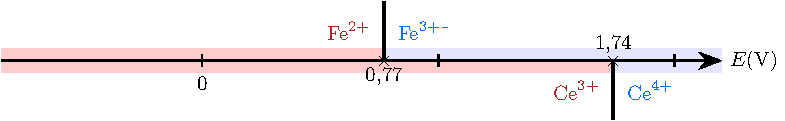
\includegraphics[width=\linewidth]{predom_2}
		}
		\vspace{-15pt}
		\captionof{figure}{Domaines disjoints.}
		\label{fig:disjoint}
	\end{center}
	\tcblower
	\begin{center}
		\sswitch{
			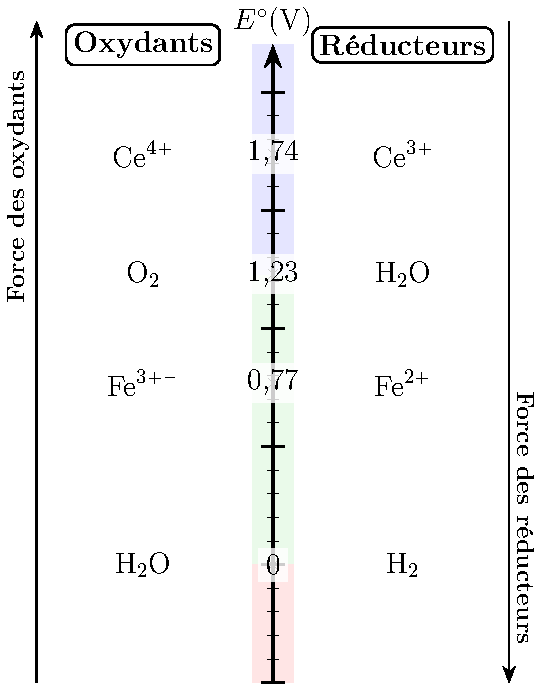
\includegraphics[width=\linewidth]{estand_fece-plain}
		}{
			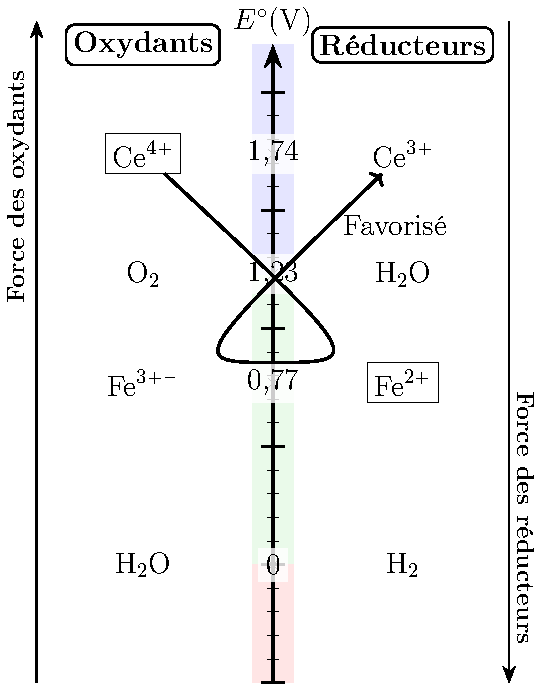
\includegraphics[width=\linewidth]{estand_fece}
		}
		\vspace{-15pt}
		\captionsetup{justification=centering}
		\captionof{figure}{\\Échelle $E^\circ$}
		\label{fig:gamma}
	\end{center}
\end{tcb*}

\subsection{Cas particuliers}
\begin{tcb*}[sidebyside, righthand ratio=.3](defi){Dismutation}
	Une réaction dans laquelle le \textbf{réactif} est \textbf{à la fois oxydant
		et réducteur} est appelée \textbf{dismutation}. On la schématise par la règle
	du gamma ci-contre, et on écrit cette réaction
	\psw{
		\[
			\ce{2A = B+C}
		\]
	}
	\vspace{-15pt}
	\tcblower
	\begin{center}
		\sswitch{
			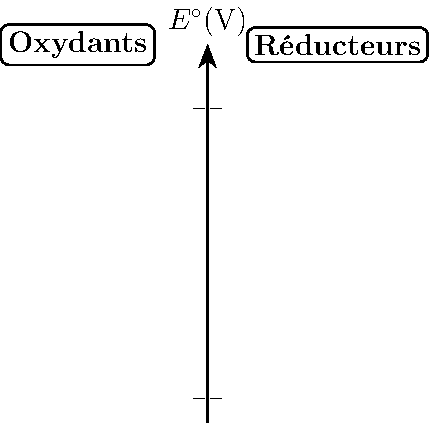
\includegraphics[width=\linewidth]{estand_dismut-plain}
		}{
			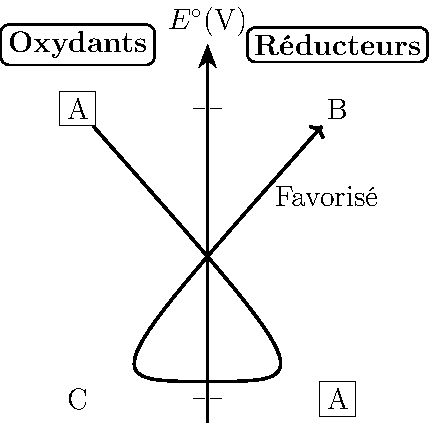
\includegraphics[width=\linewidth]{estand_dismut}
		}
	\end{center}
\end{tcb*}

\begin{tcb*}(exem)<lftt>{Dismutation du fer}
	C'est le cas de l'ion \ce{Fe^2+} qui intervient dans les couples
	\ce{Fe^3+}/\ce{Fe^2+} et \ce{Fe^2+}/\ce{Fe}~: les potentiels standard
	donnent
	\psw{
	\[
		\ce{2 {Fe}^2+_{\rm(aq)} + Fe_{\rm(s)} = 3 {Fe}^2+_{\rm(aq)}}
	\]
	}
	\vspace{-15pt}
\end{tcb*}

\begin{tcb*}[sidebyside, righthand ratio=.3](defi){Médiamutation}
	Une réaction dans laquelle le \textbf{produit} est \textbf{à la fois oxydant
		et réducteur} est appelée \textbf{médiamutation}. On la schématise par la
	règle du gamma ci-contre, et on écrit cette réaction
	\psw{
		\[
			\ce{A + B = 2C}
		\]
	}
	\vspace{-15pt}
	\tcblower
	\begin{center}
		\sswitch{
			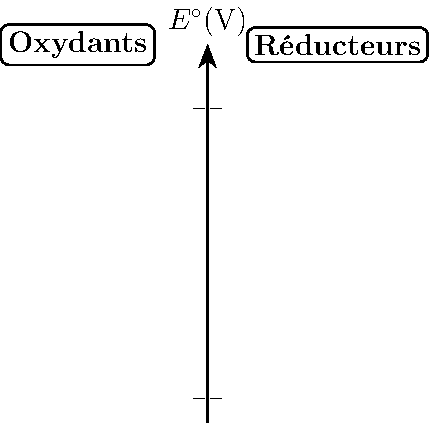
\includegraphics[width=\linewidth]{estand_mediamut-plain}
		}{
			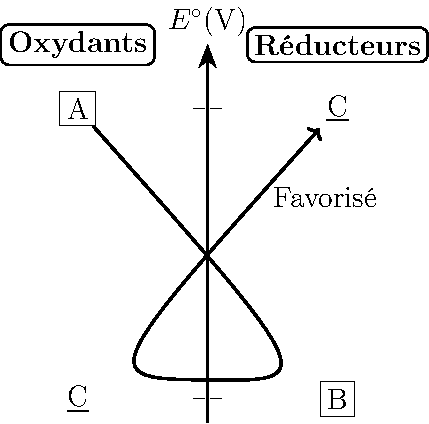
\includegraphics[width=\linewidth]{estand_mediamut}
		}
	\end{center}
\end{tcb*}

\begin{tcb*}(appl)<lftt>{Stabilité par dismutation ou médiamutation}
	Montrer que l'eau oxygénée \ce{H2O2} est instable et que l'eau est stable. On
	donne $E^\circ(\ce{H_2O_2}/\ce{H_2O}) = \SI{1.78}{V}$,
	$E^\circ(\ce{O_2}/\ce{H_2O_2}) = \SI{0.68}{V}$, $E^\circ(\ce{O_2}/\ce{H_2O}) =
		\SI{1.23}{V}$ et $E^\circ(\ce{H_2O}/\ce{H_2}) = \SI{0.0}{V}$.
	\tcblower
	\begin{isd}
		\begin{center}
			\sswitch{
				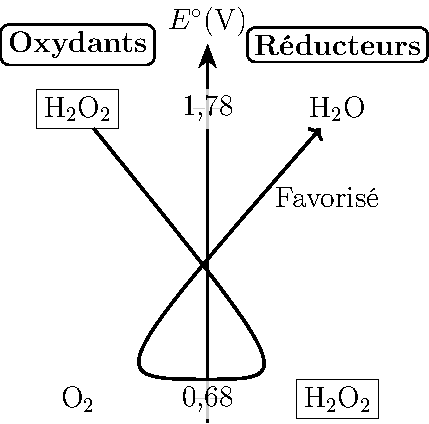
\includegraphics[width=.6\linewidth, draft=true]{estand_dismut-h2o2}
			}{
				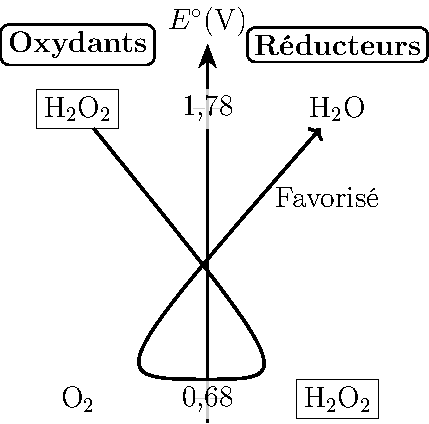
\includegraphics[width=.6\linewidth]{estand_dismut-h2o2}
			}
		\end{center}
		\psw{
			Spontanément, \ce{H2O2} réagit avec lui-même pour former \ce{H2O} et
			\ce{O2}.
		}
		\tcblower
		\begin{center}
			\sswitch{
				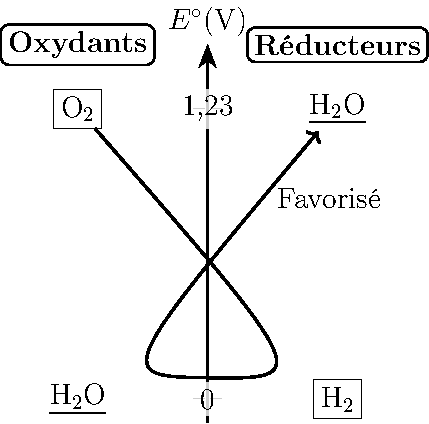
\includegraphics[width=.6\linewidth, draft=true]{estand_mediamut-h2o}
			}{
				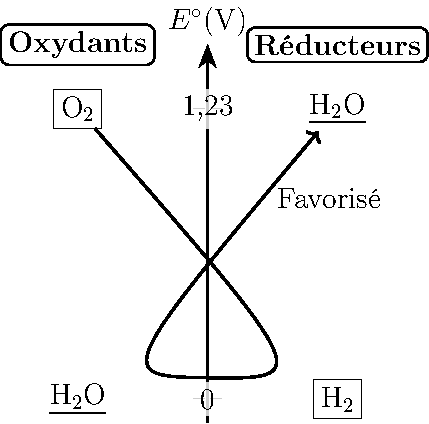
\includegraphics[width=.6\linewidth]{estand_mediamut-h2o}
			}
		\end{center}
		\psw{
			Spontanément, \ce{H2} réagit avec \ce{O2} lui-même pour former \ce{H2O}.
		}
	\end{isd}
\end{tcb*}

\subsection{Calcul de constantes d'équilibre}
\begin{tcb*}(prop){Potentiel et constante d'équilibre}
	Il y a \textbf{unicité du potentiel} en solution~: en présence de plusieurs
	couples rédox dans la solution, les potentiels des différents couples
	sont \textbf{égaux à l'équilibre}. On trouve ainsi la constante d'équilibre d'une
	réaction sans autres éléments~:
	\psw{
		\begin{gather*}
			a\ce{Ox_1} + b \ce{Red_2} = c \ce{Red_1} + d \ce{Ox_2}
			\\\Ra
			K = \frac{a_{\ce{Red_1}}{}^{c} a_{\ce{Ox_2}}{}^{d}}
			{a_{\ce{Ox_1}}{}^{a} a_{\ce{Red_2}}{}^{b}}
			\Lra
			K = \exp \left( \frac{n_{\ce{e^-},\tot}\Fc}{RT} (E_1^\circ - E_2^\circ) \right)
			\Lra
			\boxed{K = 10^{\frac{n_{\ce{e^-},\tot}}{\num{0.06}}(E_1^\circ - E_2^\circ)}}
		\end{gather*}
	}
	\vspace{-15pt}
\end{tcb*}

\begin{tcb*}(demo)<lftt>{Constante d'équilibre d'oxydoréduction}
	\begin{DispWithArrows*}[format=RrL, fleqn, mathindent=12pt, xoffset=40pt]
		\text{Égalité des potentiels~:}
		&
		\psw{E_1}
		&=
		\psw{E_2}
		\Arrow{\textsc{Nernst}}
		\\\Lra
		&
		\qquad
		\psw{
			E_1^\circ + \frac{\num{0.06}}{n_{\ce{e^-},\tot}} \log
			\frac{a_{\ce{Ox_1}{}^a}}{a_{\ce{Red_1}{}^{c}}}
		}
		&=
		\psw{
			E_2^\circ + \frac{\num{0.06}}{n_{\ce{e^-},\tot}} \log
			\frac{a_{\ce{Ox_2}{}^d}}{a_{\ce{Red_2}{}^{b}}}
		}
		\Arrow{$K =
				\frac{a_{\ce{Red_1}}{}^{c} a_{\ce{Ox_2}}{}^{d}}
				{a_{\ce{Ox_1}}{}^{a} a_{\ce{Red_2}}{}^{b}}$
		}
		\\\Lra
		&
		\psw{E_1^\circ - E_2^\circ}
		&=
		\psw{
			\frac{\num{0.06}}{n_{\ce{e^-},\tot}}
			\frac{a_{\ce{Red_1}{}^{c}} a_{\ce{Ox_2}}{}^{d}}
			{a_{\ce{Ox_1}{}^{a}} a_{\ce{Red_2}}{}^{b}}
		}
		\CArrow{$10^{(~\cdot~)}$}
		\\\Lra
		&
		\Aboxed{
			\psw{K}
			&=
			\psw{10^{\DS\frac{n_{\ce{e^-},\tot}}{\num{0.06}}(E_1^\circ - E_2^\circ)}}
		}
	\end{DispWithArrows*}
\end{tcb*}

\begin{tcb*}(impo){Calcul de constantes}
	\begin{itemize}
		\item Ne vous précipitez pas avec les formules, s'il est demandé de
		      \textbf{déterminer l'expression} il faut faire le calcul~!
		\item De même, ne vous trompez pas de sens dans la soustraction~: tout
		      dépend du sens de la réaction étudiée.
		\item On retrouvera la même chose que pour les réactions acide-base avec
		      $\pm \abs{\Delta E^\circ}$ selon que la réaction est favorisée ou non.
	\end{itemize}
\end{tcb*}

\begin{tcb*}(tool){Méthode de calcul de constantes}
	\begin{enumerate}[label=\sqenumi]
		\item Écrire les demi-réactions électroniques~;
		\item Écrire la réaction en les multipliant pour éliminer les électrons si
		      nécessaire~: on obtient $n_{\ce{e^-},\tot}$ le nombre total d'électrons échangés~;
		\item Écrire \textbf{ensuite} les formules de \textsc{Nernst} \textbf{sur
			      les équations multipliées}~;
		\item Utiliser l'unicité du potentiel à l'équilibre~;
		\item Faire apparaître et isoler $K$~;
		\item Souvent, $K$ est trop grand pour être calculé~: on calculera alors
		      $\log K$.
	\end{enumerate}
\end{tcb*}

\begin{tcb*}[breakable](appl)<lftt>{Calcul de constante d'équilibre}
	Calculer la constante de réaction entre l'eau oxygénée et l'ion permanganate.
	On donne $E_1^\circ = E^\circ(\ce{O_2}/\ce{H_2O_2}) = \SI{0.68}{V}$ et
	$E_2^\circ = E^\circ (\ce{MnO_4^-}/\ce{Mn^2+}) = \SI{1.51}{V}$.
	\tcblower
	\vspace{-15pt}
	\begin{align*}
		\beforetext{Demi-équations~:}
		\ce{
		\psw{{H_2O_2}_{\rm(aq)}}
		          & =
		\psw{{O_2}_{\rm(g)} + 2 {H}^+_{\rm(aq)} +2 e^-}
		}
		\tag{1}
		\\
		\beforetext{et}
		\ce{
		\psw{{Mn}^2+_{\rm(aq)} + 4H_2O_{\rm(l)}}
		          & =
		\psw{{MnO_4}^-_{\rm(aq)} + 8H^+_{\rm(aq)} + 5e^-}
		}
		\tag{2}
		\\
		\beforetext{Multiplication~:}
		\ce{
		\psw{5{H_2O_2}_{\rm(aq)}}
		          & =
		\psw{5{O_2}_{\rm(g)} + 10 {H}^+_{\rm(aq)} +10 e^-}
		}
		\tag*{(1') = \psw{5} $\times$ (1)}
		\\
		\beforetext{et}
		\ce{
		\psw{2{Mn}^2+_{\rm(aq)} + 8H_2O_{\rm(l)}}
		          & =
		\psw{2{MnO_4}^-_{\rm(aq)} + 16H^+_{\rm(aq)} + 10e^-}
		}
		\tag*{(2') = \psw{2} $\times$ (2)}
		\\
		\beforetext{Éq$^\circ$}
		\qquad
		\ce{
		\psw{2 {MnO_4^-}_{\rm(aq)} + 16 {H}^+_{\rm(aq)} + 5 {H_2O_2}_{\rm(aq)}}
		          & =
		\psw{2 {Mn}^2+_{\rm(aq)} + 8 {H_2O}_{\rm(l)} + 5 {O_2}_{\rm(g)} + 10 {H}^+_{\rm(aq)}}
		}
		\tag*{$\psw{(1')} - \psw{(2')}$}
		\\
		\beforetext{$\Lra$}
		\Aboxed{
		\ce{\psw{2 {MnO_4^-}_{\rm(aq)} + 6 {H}^+_{\rm(aq)} + 5 {H_2O_2}_{\rm(aq)}}}
		          & =
		\ce{\psw{2 {Mn}^2+_{\rm(aq)} + 8 {H_2O}_{\rm(l)} + 5 {O_2}_{\rm(g)}}}
		}
		\tag{3}
		\\
		\beforetext{Potentiels~:}
		\psw{E_{1'}}
		          & =
		\psw{E_1^\circ +
			\frac{\num{0.06}}{10} \log (
			\frac{p_{\ce{O_2}}^5 [\ce{H+}]^{10}}{{p^\circ}^5{c^\circ}^5[\ce{H_2O_2}]^5})
		}
		\\
		\beforetext{et}
		\psw{E_{2'}}
		          & =
		\psw{E_2^\circ +
			\frac{\num{0.06}}{10} \log (
			\frac{[\ce{MnO_4^-}]^2 [\ce{H+}]^{16}}{{c^\circ}^{16}[\ce{Mn^2+}]^2})
		}
		\\
		\beforetext{Équilibre $\Lra E_{1'} = E_{2'} \Lra$}
		\psw{E_2^\circ - E_1^\circ}
		          & =
		\psw{
			\frac{\num{0.06}}{10}
			\left(\log(\frac{p_{\ce{O_2}}^5 [\ce{H+}]^{10}}{{p^\circ}^5 {c^\circ}^5 [\ce{H_2O_2}]^5})
			-
			\log(\frac{[\ce{MnO_4^-}]^2 [\ce{H+}]^{16}}{{c^\circ}^{16}[\ce{Mn^2+}]^2})\right)
		}
		\\
		\beforetext{$\Lra$}
		\psw{E_2^\circ - E_1^\circ}
		          & =
		\psw{
			\frac{\num{0.06}}{10} \log (
			\frac{p_{\ce{O_2}}^5 [\ce{Mn^2+}]^2 {c^\circ}^{11}}
			{{p^\circ}^5[\ce{H_2O_2}]^5[\ce{MnO_4^-}]^2 [\ce{H+}]^6}
			)
			=
			\frac{\num{0.06}}{10} \log K
		}
		\\
		\beforetext{$\Lra$}
		\Aboxed{
			\psw{\log K}
		          & =
			\psw{
				\frac{10}{\num{0.06}} \left(
				E^\circ \left( \ce{MnO_4^-}/\ce{Mn^2+} \right) -
				E^\circ \left( \ce{O_2}/\ce{H_2O_2} \right) \right)
			}
		}
		\\
		\beforetext{Soit}
		\Aboxed{K & = \psw{10^{\num{140}}}}
	\end{align*}
\end{tcb*}

\section{Piles électrochimiques}
Par essence, les réactions d'oxydoréduction sont le siège d'un transfert
d'électrons du \textbf{réducteur vers l'oxydant}, par exemple~:
\vspace{-15pt}
\psw{
\[
	\ce{{Cu}^2+_{\rm(s)} + Zn_{\rm(s)} = Cu_{\rm(s)} + {Zn}^2+_{\rm(aq)}}
\]
}%
Ainsi, en imposant que le transfert se fasse par un \textbf{circuit électrique
	extérieur} à la solution, on pourra mettre en évidence ce transfert par
l'utilisation d'un voltmètre, et donc et utiliser cette énergie en réalisant une
pile~!

\subsection{Présentation}
\begin{center}
	\sswitch{
		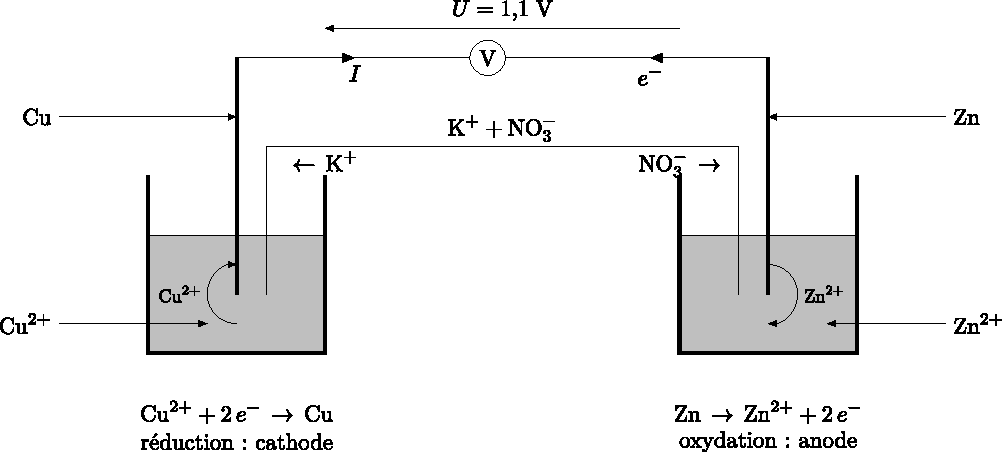
\includegraphics[width=\linewidth, draft=true]{pile_cu-zn}
	}{
		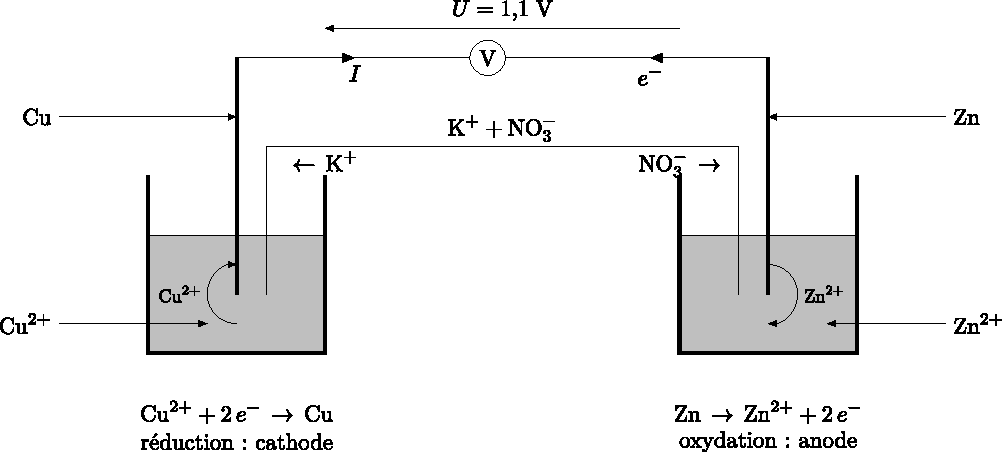
\includegraphics[width=\linewidth]{pile_cu-zn}
	}
	\vspace{-15pt}
	\captionof{figure}{Présentation de la pile \textsc{Daniell}\protect\ftn{Constituée
			par le chimiste britannique John \textsc{Daniell} en 1836}}
	\label{fig:daniell}
\end{center}

\begin{tcb*}(defi){Piles électrochimiques}
	Une pile électrochimique est constituée de~:
	\begin{itemize}
		\bitem{Une demi-pile}~: \psw{constituée par deux espèces d'un couple rédox
			en contact}
		\bitem{Une électrode}~: \psw{le métal de la demi-pile qui plonge en
			solution~: transfert les \textbf{électrons au sein} de la demi-pile}
		\bitem{Un pont salin}~: \psw{un tube contenant des ions en solution~:
			transfert les \textbf{charges entre} les demi-piles (ferme le circuit)}
	\end{itemize}
	Dans chaque demi-pile se produit un processus d'oxydation ou de réduction~:
	\begin{itemize}
		\bitem{La cathode} est le siège de \xul{\psw{la réduction}}~;
		\bitem{L'anode} est le siège de \xul{\psw{l'oxydation}}.
	\end{itemize}
\end{tcb*}

\begin{tcb*}(exem)<lftt>{Demi-piles usuelles}
	\noindent
	\hfill
	\begin{minipage}[c]{.30\linewidth}
		\begin{center}
			\sswitch{
				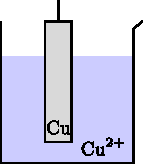
\includegraphics[width=.5\linewidth, draft=true]{piledemi_Cu}
			}{
				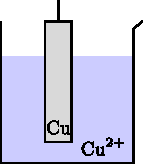
\includegraphics[width=.5\linewidth]{piledemi_Cu}
			}
			\\
			Demi-pile \ce{Cu^2+}/\ce{Cu}
			\\
			\psw{$\ce{{Cu}^2+_{\rm(aq)} + 2e^- = Cu_{\rm(s)}}$}
		\end{center}
	\end{minipage}
	\hfill
	\begin{minipage}[c]{.30\linewidth}
		\begin{center}
			\sswitch{
				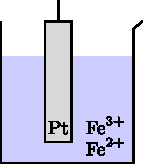
\includegraphics[width=.5\linewidth, draft=true]{piledemi_Fe}
			}{
				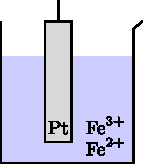
\includegraphics[width=.5\linewidth]{piledemi_Fe}
			}
			\\
			Demi-pile \ce{Fe^3+}/\ce{Fe^2+}
			\\
			\psw{$\ce{{Fe}^3+_{\rm(aq)} + e^- = {Fe}^2+_{\rm(aq)}}$}
		\end{center}
	\end{minipage}
	\hspace*{\fill}
	\begin{minipage}[c]{.30\linewidth}
		\begin{center}
			\sswitch{
				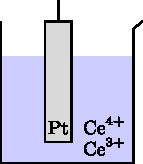
\includegraphics[width=.5\linewidth, draft=true]{piledemi_Ce}
			}{
				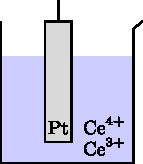
\includegraphics[width=.5\linewidth]{piledemi_Ce}
			}
			\\
			Demi-pile \ce{Ce^4+}/\ce{Ce^3+}
			\\
			\psw{$\ce{{Ce}^4+_{\rm(aq)} + e^- = {Ce}^3+_{\rm(aq)}}$}
		\end{center}
	\end{minipage}
	\smallbreak
	Si l'une des espèces du couple n'est pas métallique et donc ne peut être
	l'électrode, on utilisera une électrode faite en un autre métal peu oxydable
	afin d'assurer l'échange d'électrons au sein de la solution, par exemple le
	platine.
\end{tcb*}

\begin{tcb*}(ror){Production et réception des électrons}
	Les électrons sont produits par \xul{\psw{l'oxydation}}, donc
	\xul{\psw{à l'anode}}, et sont reçus \textit{via} \xul{\psw{la réduction}},
	donc \xul{\psw{à la cathode}}.
\end{tcb*}

\begin{tcb*}(nota)<lftt>{Pile schématique}
	Schématiquement et sur l'exemple de la pile \textsc{Daniell}, on peut les
	représenter par
	\psw{
		\[
			\ominus~\ce{Zn}|\ce{Zn^2+}||\ce{Cu^2+}|\ce{Cu}~\oplus
		\]
	}
	\vspace{-30pt}
\end{tcb*}

\subsection{Force électromotrice}
\begin{tcb*}(defi){Potentiel d'électrode et f.e.m.}
	La force électromotrice (f.e.m.) $e$ est la \textbf{tension} mesurée aux
	bornes d'une pile \textbf{qui ne débite pas}~; elle s'exprime donc en
	\xul{\psw{volts}}, telle que
	\psw{
		\[
			e = V_+ - V_- = E(\ce{Ox_1}/\ce{Red_1}) - E(\ce{Ox_2}/\ce{Red_2})
		\]
	}%
	Avec $E_1$ et $E_2$ les \textbf{potentiels d'électrode} des couples. Elle
	traduit le \textbf{déséquilibre chimique} d'une réaction spontanée
	envisageable.
\end{tcb*}

\begin{tcb*}(appl)<lftt>{Calcul de la f.e.m.\ de la pile \textsc{Daniell}}
	\noindent
	\begin{minipage}[c]{.48\linewidth}
		On prépare une pile \textsc{Daniell} avec les concentrations $c_1$ en ions
		$\ce{Cu^2+}$ et $c_2$ en ions $\ce{Zn^2+}$, et on relie les électrodes par une
		résistance (ou une ampoule). Au début de l'établissement du courant, quelle
		est la tension de la pile~?
	\end{minipage}
	\hfill
	\begin{minipage}[c]{.48\linewidth}
		\vspace{0pt}
		\begin{center}
			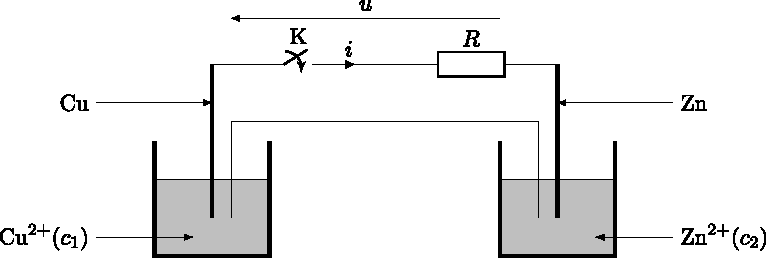
\includegraphics[width=\linewidth]{pile_fem-R}
			\label{fig:fem_R}
		\end{center}
	\end{minipage}
	On donne $E^\circ \left( \ce{Cu^2+}/\ce{Cu} \right) = \SI{0.34}{V}$,
	$E^\circ \left( \ce{Zn^2+}/\ce{Zn} \right) = \SI{-0.76}{V}$ et $c_1 = c_2 =
		\SI{0.01}{mol.L^{-1}}$.
	\tcblower
	\vspace{-15pt}
	\psw{
		\begin{gather*}
			E_G = E^\circ \left( \ce{Cu^2+}/\ce{Cu} \right) + \frac{\num{0.06}}{2}
			\log [\ce{{Cu}^2+_{\rm(aq)}}]_i = \SI{0.28}{V}
			\\
			E_D = E^\circ \left( \ce{Zn^2+}/\ce{Zn} \right) + \frac{\num{0.06}}{2}
			\log [\ce{{Zn}^2+_{\rm(aq)}}]_i = \SI{-0.82}{V}
			\\
			\Lra
			\boxed{u(0) = e = \abs{E_D - E_G}}
			\Ra
			\xul{e = \SI{1.10}{V}}
		\end{gather*}
	}
	\vspace{-15pt}
\end{tcb*}

\begin{tcb*}[breakable](defi){Électrodes de référence}
	On ne peut accéder expérimentalement au potentiel d'une unique électrode, on
	ne mesure que des différences de potentiel. On utilise pour cela des
	électrodes de référence dont on connaît les potentiels par définition. On
	trouve~:
	\begin{isd}[sidebyside align=top]
		\begin{itemize}
			\bitem{L'électrode standard à hydrogène (ESH)}~: il s'agit de la référence
			absolue, siège du couple de l'eau
			$\ce{{H}^+_{\rm(aq)}}/\ce{{H_2}_{\rm(g)}}$~:
			\[
				\ce{2 {H}^+_{\rm(aq)} + 2e^- = {H_2}_{\rm(g)}}
			\]
			avec $[\ce{H^+}] = c^\circ = \SI{1}{mol.L^{-1}}$~; $p_{\ce{H_2}} = p^\circ
				= \SI{1}{bar}$~; fil de platine en solution.
			Ainsi,
			\[
				\boxed{E\ind{ESH} = \SI{0.00}{V}}
			\]
		\end{itemize}
		\tcblower
		\begin{itemize}
			\bitem{L'électrode au calomel saturé (ECS)}~: dans la pratique, on utilise
			souvent cette électrode, siège du couple~:
			\[
				\ce{{Hg_2Cl_2}_{\rm(s)} + 2e^- = 2 Hg_{\rm(s)} + 2 {Cl}^-_{\rm(aq)}}
			\]
			Pour garder la concentration en \ce{Cl^-} constante, on sature la solution
			en chlorure de potassium $\ce{KCl}_{\rm(s)}$, d'où son nom. Ainsi,
			\[
				\boxed{E\ind{ECS} = \SI{0.24}{V}}
			\]
		\end{itemize}
	\end{isd}
	\begin{center}
		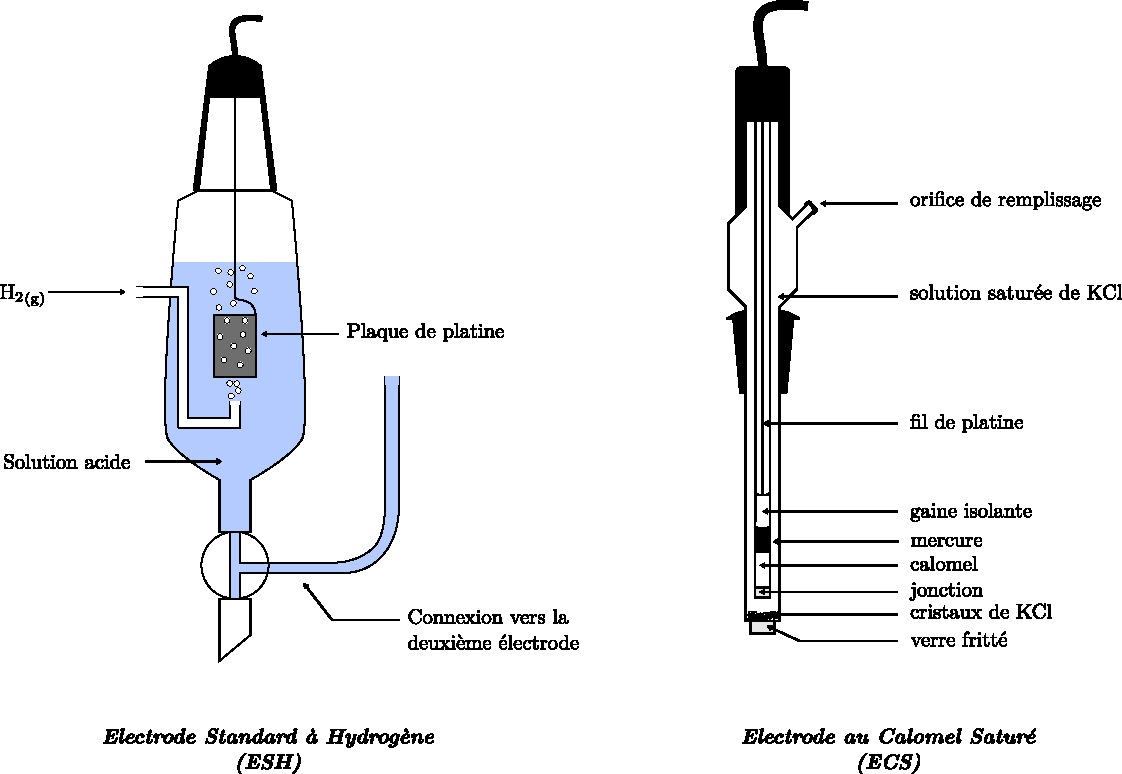
\includegraphics[width=.7\linewidth]{esh_ecs}
	\end{center}
	\begin{itemize}
		\item On trouve également une électrode au chlorure d'argent avec le
		      couple $\ce{AgCl_{\rm(s)}}/\ce{Ag_{\rm(s)}}$ avec une solution saturée
		      en ions $\ce{Cl^-}$.
	\end{itemize}
\end{tcb*}

\subsection{Charge totale d'une pile}

Tant que la pile débite, la réaction se fait dans le sens direct jusqu'à
atteindre l'équilibre chimique, i.e. $Q_{r,f} = K^\circ$, ou jusqu'à rupture
d'équilibre. Durant ce temps total, elle aura délivré une certaine quantité
d'électricité. On trouve alors~:
\begin{tcb*}(prop){Quantité d'électricité d'une pile}
	La quantité d'électricité $Q$ d'une pile est la charge qu'elle peut délivrer
	jusqu'à épuisement, et s'exprime~:
	\psw{
		\[
			\boxed{Q = n \xi\ind{eq}\Fc}
		\]
	}%
	avec $\Fc = \Nc_A e \approx \SI{96500}{C.mol^{-1}}$ la charge électrique dans
	une mole d'électrons.
\end{tcb*}

\begin{tcb*}(demo)<lftt>{Quantité d'électricité d'une pile}
	\begin{center}
		\def\rhgt{0.50}
		\centering
		\begin{tabularx}{\linewidth}{|l|c||YdYdYdY||Y|}
			\hline
			\multicolumn{2}{|c||}{
				$\xmathstrut{\rhgt}$
			\textbf{Équation}}   &
			\psw{$a\ce{Ox_1}$}   & $+$       &
			\psw{$b\ce{Red_2}$}  & $=$       &
			\psw{$c\ce{Red_1}$}  & $+$       &
			\psw{$d\ce{Ox_2}$}   &
			\psw{$\ce{e^-}$}                   \\
			\hline
			$\xmathstrut{\rhgt}$
			Initial              & $\xi = 0$ &
			\psw{$n_a$}          & \vline    &
			\psw{$n_b$}          & \vline    &
			\psw{$n_c$}          & \vline    &
			\psw{$n_d$}          &
			\psw{$0$}
			\\
			\hline
			$\xmathstrut{\rhgt}$
			Interm.              & $\xi$     &
			\psw{$n_a - a\xi$}   & \vline    &
			\psw{$n_b - b\xi$}   & \vline    &
			\psw{$n_c + c\xi$}   & \vline    &
			\psw{$n_d + d\xi$}   &
			\psw{$n_{\ce{e^-},\tot}\xi$}       \\
			\hline
			$\xmathstrut{\rhgt}$
			Final                & $\xi_f$   &
			\psw{$n_a - a\xi_f$} & \vline    &
			\psw{$n_b - b\xi_f$} & \vline    &
			\psw{$n_c + c\xi_f$} & \vline    &
			\psw{$n_d + d\xi_f$} &
			\psw{$n_{\ce{e^-},\tot}\xi_{f}$}   \\
			\hline
		\end{tabularx}
	\end{center}
	% \psw{
	%       Avec $n = 2$ le nombre d'électrons échangés~: à chaque étape, \ce{Zn}
	%     produit deux électrons à l'anode qui vont vers la cathode, où \ce{Cu^2+} les
	%     reçoit pour former du cuivre. Ainsi, pour $\xi_f$ moles de $\ce{Cu^2+}$ ou
	%     $\ce{Zn}$ réagissant, $2\xi_{f}$ moles d'électrons circulent.
	% }
	\vspace{-15pt}
	\begin{gather*}
		\beforetext{Ainsi,}
		\psw{
		Q =
		\xunderbracket{n_{\ce{e^-},\tot} \xi_f}_{\si{mol}}
		\times
		\xunderbracket{\Nc_A}_{\si{mol^{-1}}}
		\times
		\xunderbracket{e}_{\si{C}}
		\Lra
		\boxed{Q = n \xi_f \Fc}
		}
		\vspace{-15pt}
	\end{gather*}
\end{tcb*}

\begin{tcb*}(appl)<lftt>{Charge de la pile \textsc{Daniell}}
	Soit une pile \textsc{Daniell} constituée de $c_1 =
		c_2 = c = \SI{0.01}{mol.L^{-1}}$ de \ce{Cu^2+} et de \ce{Zn^2+} ayant chacun
	un volume $V = \SI{100}{mL}$. Déterminer sa charge totale en coulomb d'abord,
	puis en \si{A.h} ensuite.
	\tcblower
	\begin{center}
		\def\rhgt{0.50}
		\centering
		\begin{tabularx}{\linewidth}{|l|c||YdYdYdY||Y|}
			\hline
			\multicolumn{2}{|c||}{
				$\xmathstrut{\rhgt}$
			\textbf{Équation}}             &
			\psw{$\ce{{Ce}^2+_{\rm(aq)}}$} & $+$       &
			\psw{$\ce{Zn_{\rm(s)}}$}       & $\ra$     &
			\psw{$\ce{Cu_{\rm(s)}}$}       & $+$       &
			\psw{$\ce{{Zn}^2+_{\rm(aq)}}$} &
			\psw{$\ce{e^-}$}                             \\
			\hline
			$\xmathstrut{\rhgt}$
			Initial                        & $\xi = 0$ &
			\psw{$n_1$}                    & \vline    &
			\psw{excès}                    & \vline    &
			\psw{excès}                    & \vline    &
			\psw{$n_2$}                    &
			\psw{$0$}
			\\
			\hline
			$\xmathstrut{\rhgt}$
			Final                          & $\xi_f$   &
			\psw{$n_1 - \xi_{f}$}          & \vline    &
			\psw{excès}                    & \vline    &
			\psw{excès}                    & \vline    &
			\psw{$n_2 + \xi_{f}$}          &
			\psw{$2\xi_{f}$}                             \\
			\hline
		\end{tabularx}
	\end{center}
	\psw{
		Dans ce cas, la réaction est \textbf{totale}~:
		\begin{gather*}
			\log K = \frac{2}{\num{0.06}} \abs{\Delta E^\circ} \approx 37
			\\\Ra
			\xi_f = \xi\ind{max} = cV = \SI{1e-3}{mol}
			\Ra
			\boxed{Q = 2\xi_f \Fc}
			\Ra
			\xul{Q = \SI{193}{C} \approx \SI{0.05}{A.h}}
		\end{gather*}
	}
	\vspace{-30pt}
\end{tcb*}

\end{document}
